\section*{Preface}
In this chapter, we discuss performance of AIBs using two-dimensional molybdenum dichalcogenides such as \ce{MoS2}, \ce{MoSe2} and MoSSe in their bulk and nano form, as cathodes for AIBs attempt to establish their mechanism. We explored different molybdenum dichalcogenide-based cathodes and their mechanism of energy storage. We expected that two-dimensional (2D) layered materials that support intercalation of charged species might be suitable as active cathode materials in AIBs. 
\pagebreak
\chapter{Molybdenum dichalcogenides as cathodes for rechargeable AIBs} % Main chapter title

\label{chap4} % For referencing the chapter elsewhere, use \ref{Chapter1} 

\section{Theory and background}
Transition metal dichalcogenides (TMDs) have a strong in-plane covalent bonding and weaker van der Waals (vdW) bonds exist between any two layers, which is quite similar to graphene layers in graphite. The 2D structure facilitates intercalation of ions within these layers. Molybdenum dichalcogenides not only provide redox variability but also a high theoretical capacity (600-1200 mAh g$^{-1}$). The intercalation voltage observed with \ce{MX2}, where M = Mo, W, Ti, etc. and X = S and Se, is high ($\approx$ 2.0 V). The mechanism that TMDs follow is based on intercalation as well as conversion. 
Molybdenum dichalcogenides (\ce{MoX2} where X=S, Se or Te) display similar properties as graphite. They have a 2D-layered structure, which allows intercalation of ions and are electrically conductive. Lower volumetric expansion on cycling is an advantage these materials have over graphitic cathodes \cite{liang_rechargeable_2011, huang_molybdenum_2019}. Amongst various transition metal chalcogenides, \ce{MoS2} has been extensively studied as a cathode for rechargeable batteries \cite{li_mos2_2004, zhu_fast_2015}, making them attractive candidates for AIB cathodes. In 2015, Geng \textit{et al.} found that \ce{Al^3+} ions fully intercalated into chevrel phase \ce{Mo6S8} with the cations occupying two different sites in the crystal lattice \cite{geng_reversible_2015}. This mechanism was called the 'rocking chair' mechanism where charge carrying species shuttled back and forth between intercalating electrodes during cycles while the overall electrolyte concentration remains constant. The discharging and charging reactions at the anode (equation 1) and cathode (equation 2) were proposed as follows:

\begin{align}
          \ce{Al + 7AlCl4^-} &\rightleftharpoons 4\ce{Al2Cl7^- + 3e^-}\\
\ce{8AlCl7^- + 6e^- + Mo6S8 &\rightleftharpoons Al2Mo6S8 + 14AlCl4^-}
\end{align}

Three years later, Li \textit{et al.} prepared \ce{MoS2} microspheres by a simple hydrothermal method \cite{li_rechargeable_2018}. They proposed a similar mechanism where \ce{Al^3+} ions inserted into the electrode accompanied by a phase transformation at the electrode interface. Li and his group confirmed this phase-transition by using \textit{ex-situ} XPS and XRD etching techniques. The reaction equations for this battery system at the cathode (equation 3) and anode (equation 4) were proposed as follows:
\begin{align}
    \ce{MoS2 + x\ce{Al^{3+}}  + 3x\ce{e-} &\rightleftharpoons Al_xMoS2}\\
    \ce{Al} + 7x\ce{AlCl4-} &\rightleftharpoons 4x\ce{Al2Cl7-} + 3x\ce{e-}
\end{align}

In general, these cells showed low energy density and had reversibility issues in the redox processes. It has been reported that transition metal dichalcogenide electrodes tend to transition from a 2H phase into a more conducting 1T phase when used in a battery \cite{fan_hybrid_2017}. A hybrid \ce{Mg^{2+}}/\ce{Li+} cell was tested using bulk \ce{MoS2} as a cathode material. During cyclic voltammetry (CV) scans, the authors associated the first cathodic peak, with a phase transition. 2H phase \ce{MoS2} was converted to 1T phase during initial ion intercalation. This seems to be a common phenomenon for molybdenum dichalcogenides, since Li \textit{et al.} observed similar transitions in sodium ion batteries \cite{li_enhancing_2015}. It mostly takes place during the first cycle and since the phase change is irreversible, it can be detected in a cyclic voltammogram.

This chapter documents a range of 2D molybdenum dichalcogenides including \ce{MoS2}, \ce{MoSe2} and \ce{MoSSe}, as cathodes for non-aqueous AIBs. Our unpublished, preliminary density functional theory (DFT) calculations indicated a significant decrease in inter-layer spacing of these materials when \ce{Al^3+} cations were assumed to intercalate (owing to the very high charge density of \ce{Al^3+}). Therefore, we propose intercalation of structurally distorted \ce{AlCl4-} anions into the cathode layers. Surprisingly we found that \ce{MoSe2}-based cathodes performed different and better than all of the other molybdenum dichalcogenides.

\section{Experimental methods}
Same as discussed in Chapter 3.

\section{Results and Discussion}
Figure \ref{Figures/chap4fig:S1} shows the crystal structure of \ce{MoX2} where X is sulfur (S) and/or selenium (Se). The material has two vacant sites for intercalation --- M1 and M2. M1 denotes the spaces in between the X-Mo-X atoms, whereas M2 represents the space created between the \ce{MoX2} layers as shown in Figure \ref{Figures/chap4fig:S1} a). The inter-layer distance in \ce{MoX2} is 6.3 \AA\ with a gallery height of 3 \AA. The layers are held together by weak van der Waals (vdW) forces. M2 presents an open network and provides various interstitial sites for intercalation. Since \ce{AlCl4-} ions are 5.28 \AA\ in diameter, as reported by Takahashi {\it et al.} \cite{takahashi_niv2o5nh2o_2005}, they undergo some distortion during intercalation to fit into these layers. Our preliminary results showed that \ce{Al^{3+}} would \lq contract\rq\ the \ce{MoX2} layers when trying to intercalate, making \ce{AlCl4-} anion intercalation more likely. Also, the triply charged \ce{Al^{3+}} cation has to overcome strong electrostatic forces from the \ce{S^{2-}} or \ce{Se^{2-}} anion network in order to enter, making the intercalation process slow and most likely not reversible. Therefore, we propose intercalation of \ce{AlCl4-} anions from the electrolyte into M2 sites of \ce{MoX2} during charge. Galvanostatic cycles, cyclic voltammetry (CV), X-Ray diffraction (XRD), Raman spectra and X-Ray Photoelectron Spectroscopy (XPS) results discussed later, strongly support our claim of a reversible intercalation process especially in \ce{MoSe2}.

\begin{figure}
  \centering
  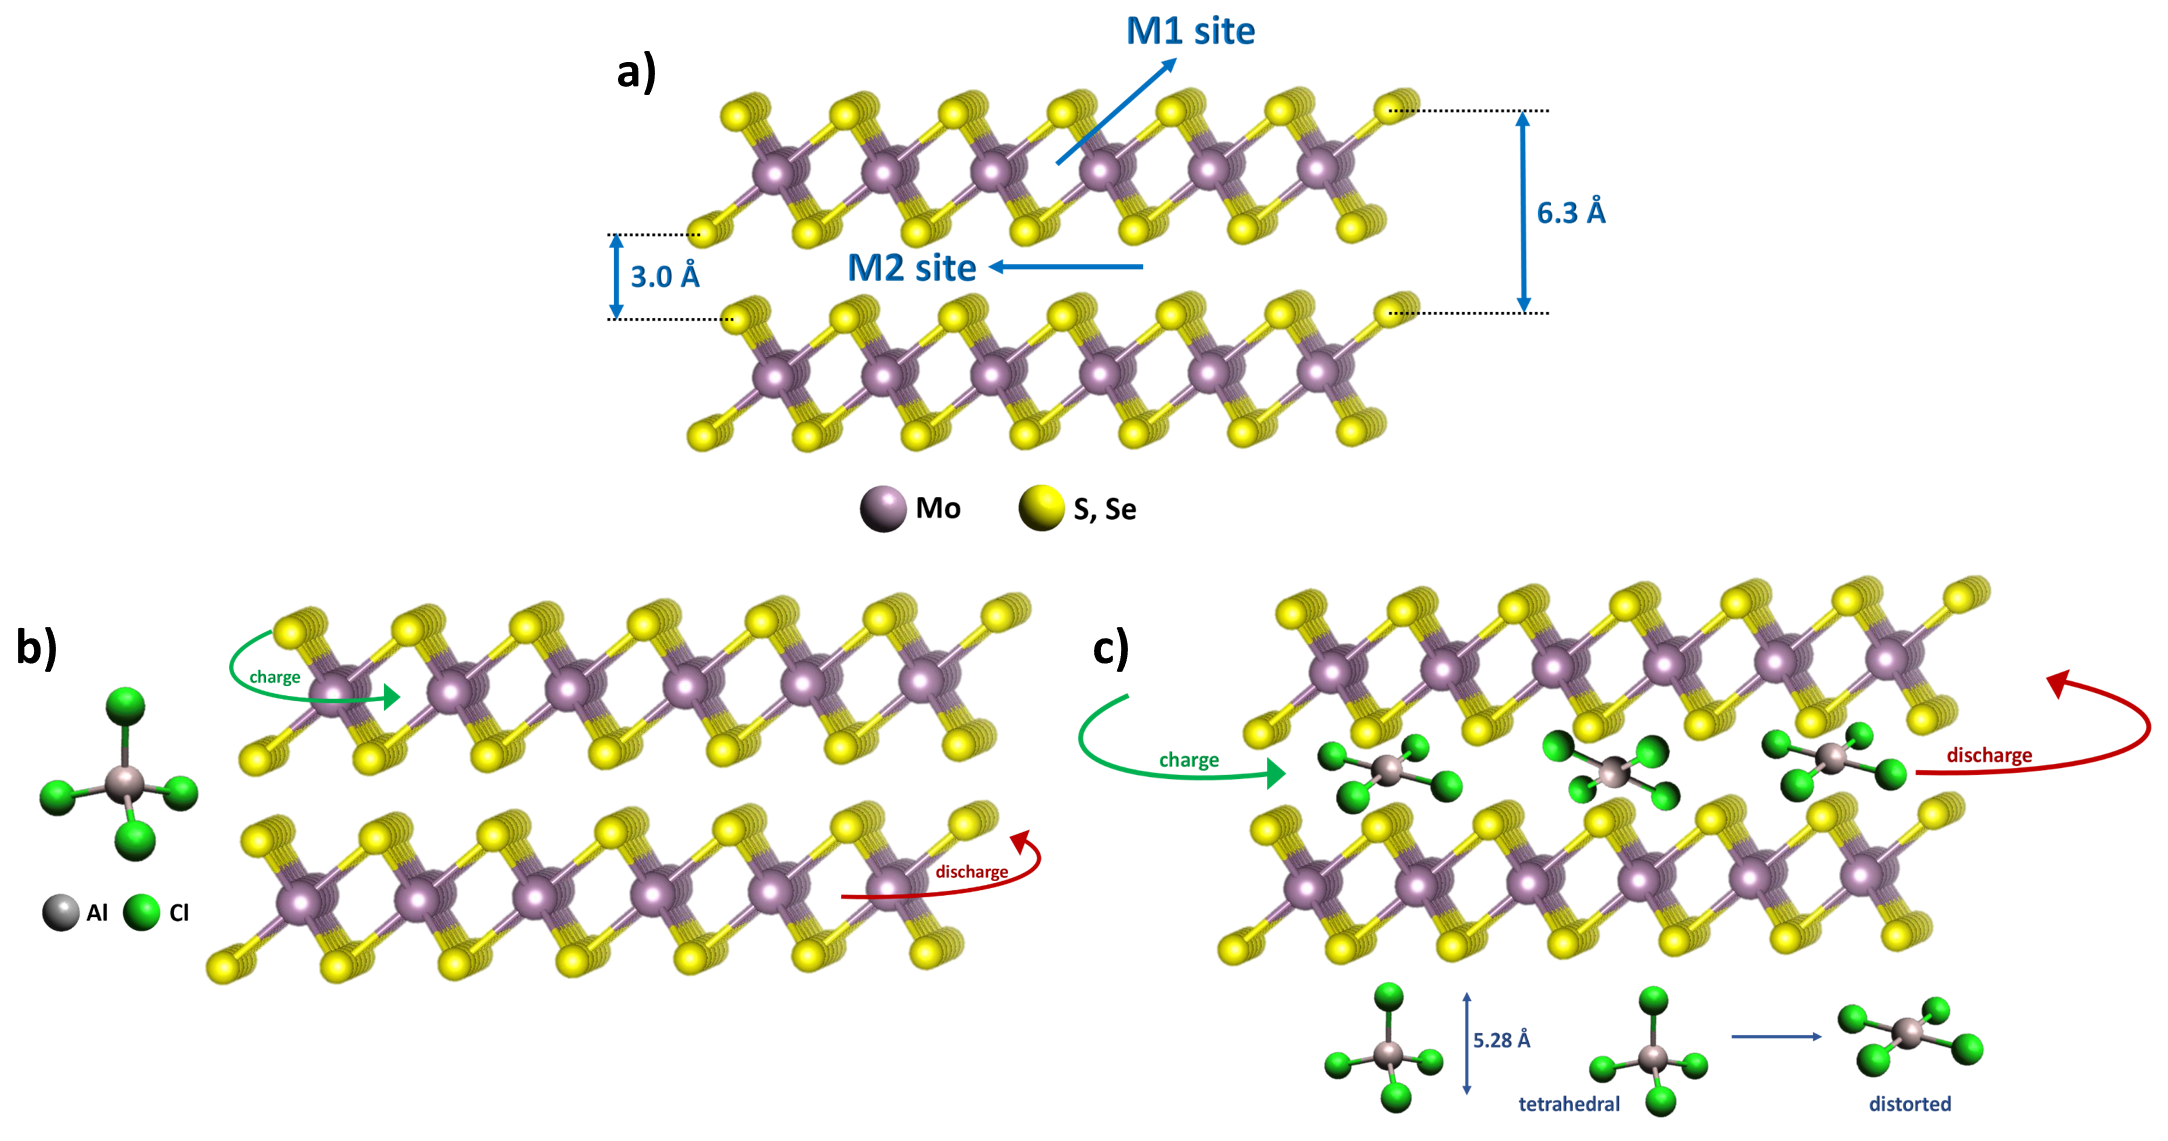
\includegraphics[width=\textwidth]{Figures/chap4fig/S1}
  \caption{Schematic representation of a) a \ce{MoX2} crystal structure with possible intercalation sites at M1 and M2 b) intercalation at M1 site and c) intercalation at M2 site.}
  \label{Figures/chap4fig:S1}
\end{figure}

\begin{figure}[htb!]
\centering
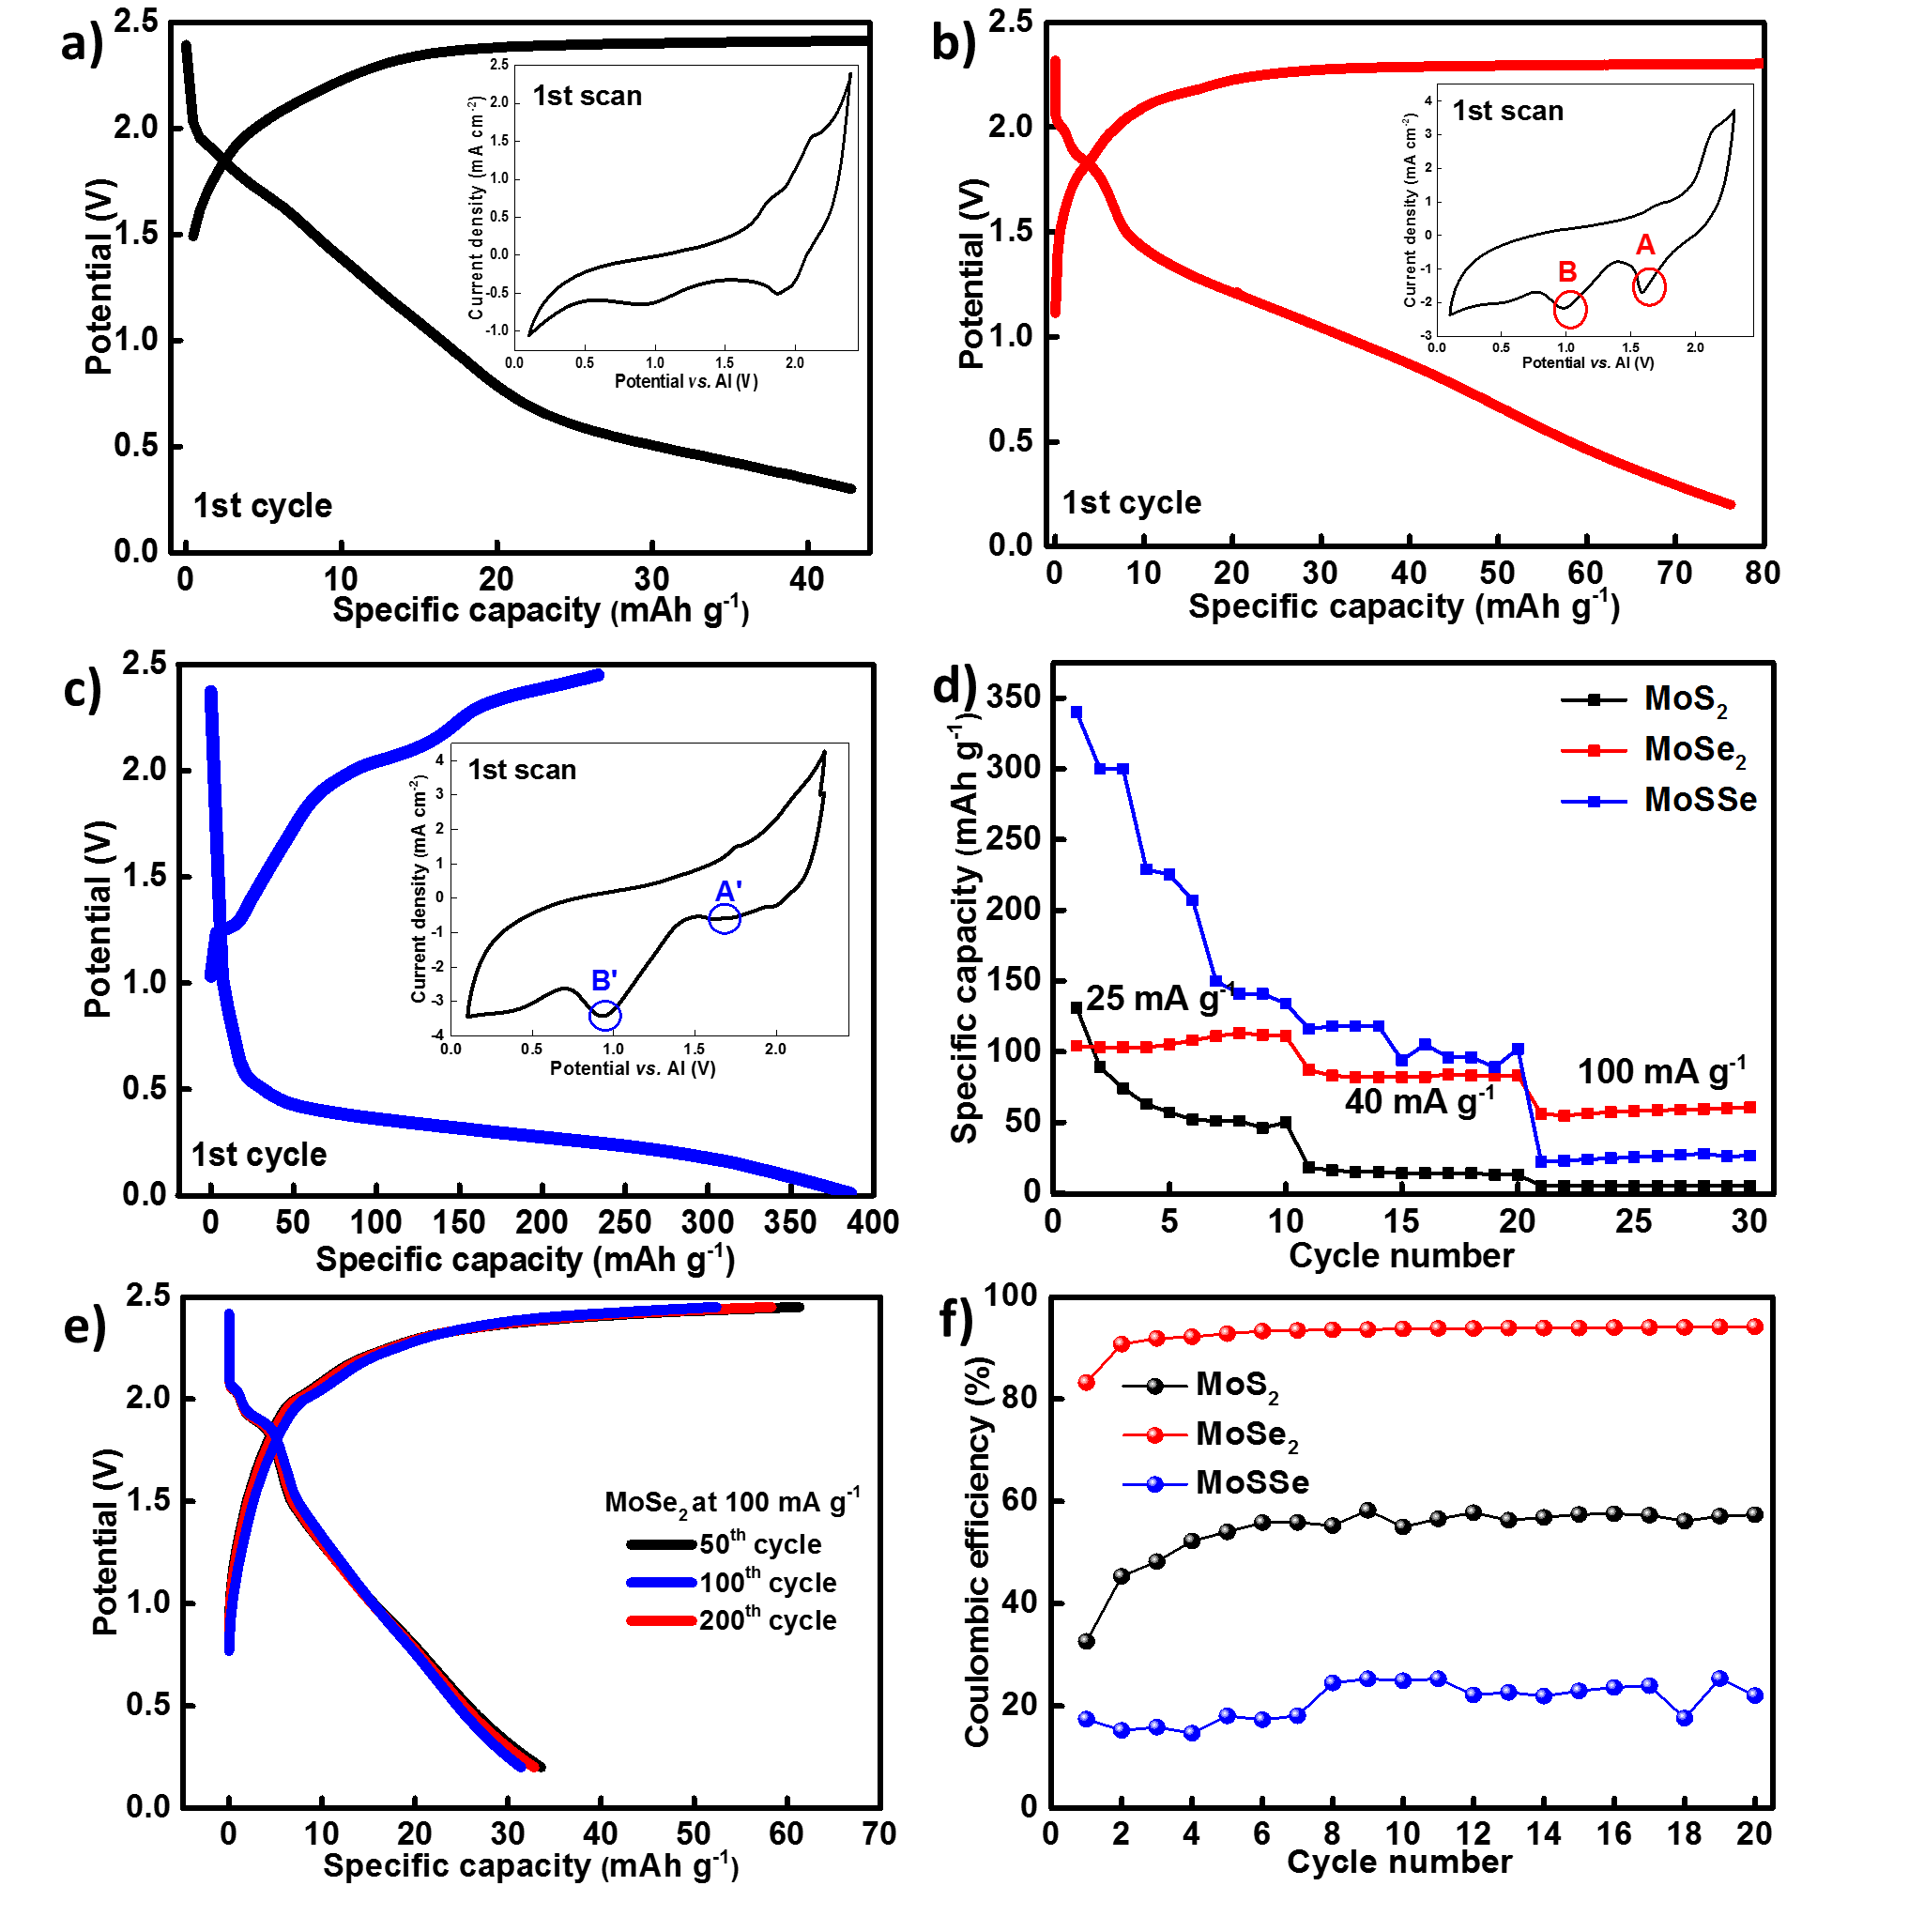
\includegraphics[width=\textwidth]{Figures/chap4fig/MoX2CDCCV}
\caption{First charge/discharge curve at 40 mA g$^{-1}$ for a) \ce{MoS2}, b) \ce{MoSe2} and c) MoSSe. d) Specific capacities of \ce{MoS2}, \ce{MoSe2} and MoSSe at current rates of 25, 40 and 100 mA g$^{-1}$. e)First CV scan of \ce{MoS2}, f) \ce{MoSe2} and g) MoSSe at a scan rate of 10 mV s$^{-1}$ in an aluminium-ion battery against Al reference electrode.}
\label{Figures/chap4fig:MoX2CDCCV}
\end{figure} 

Figure \ref{Figures/chap4fig:MoX2CDCCV} a)--c) shows the charge/discharge cycles (CDCs) for \ce{MoS2}, \ce{MoSe2} and MoSSe at a current rate of 40 mA g$^{-1}$. The discharge capacity of Al/\ce{MoS2} in its first cycle was found at $\sim$45 mAh g$^{-1}$, Figure \ref{Figures/chap4fig:MoX2CDCCV} a). Comparing this with its first CV scan (Figure \ref{Figures/chap4fig:MoX2CDCCV} g), a good correlation between the discharge voltage plateau and reduction peaks, and other redox features was found. With discharge plateaus at 1.9 V and 1.7 V, the first CV scan for \ce{MoSe2} displayed two reduction peaks at 1.65 V (point A) and 1.0 V (point B), Figures \ref{Figures/chap4fig:MoX2CDCCV} b) and \ref{Figures/chap4fig:MoX2CDCCV} h). The peak at 1.0 V suggested an irreversible reaction since this peak was absent in the following scans. Based on this, we agree with Li \textit{et al.}'s interpretation and attributed this peak to an irreversible phase transition \cite{li_enhancing_2015}. During this transition, the semi-conducting 2H phase converted into a more metallic 1T phase. This transition seemed to increase the interlayer spacing of \ce{MoSe2} by reducing the vdW forces that exist between the two layers \cite{fan_hybrid_2017}. Al/MoSSe cells showed three distinct plateaus during charging at 1.2 V, 2.0 V and 2.3 V in its first cycle, with a discharge plateau at 0.5 V shown in Figure \ref{Figures/chap4fig:MoX2CDCCV} c). Capacities of all molybdenum dichalcogenides were recorded at different current rates of 25, 40 and 100 mA g$^{-1}$, and displayed in Figure \ref{Figures/chap4fig:MoX2CDCCV} d). Since \ce{MoSe2} displayed stable specific capacities at all current rates, we recorded further 200 cycles at the highest current rate of 100 mA g$^{-1}$. A highly reversible electrochemical reaction was observed since the capacity remained at 30-32 mAh g$^{-1}$ after 200 cycles (Figure \ref{Figures/chap4fig:MoX2CDCCV} e)). The presence of multiple charging plateaus in MoSSe might correspond to various oxidation processes occurring when \ce{AlCl4-} interacts individually with S and Se atoms. The first CV scan in Figure \ref{Figures/chap4fig:MoX2CDCCV} i) showed an irreversible reduction potential at 0.9 V, point B', like \ce{MoSe2}, implying a similar phase transition. It seems MoSSe undergoes a lattice distortion and the material loses its long range order after converting to its 1T phase. This might be the reason why the cells fail to deliver a stable capacity.

CV of a blank cell with an uncoated Mo foil (Figure inset\ \ref{Figures/chap4fig:fig2} a)) showed that the current collector did not contribute to the cell's capacity. Both \ce{MoS2} and \ce{MoSe2} have similar interlayer distance (6.3 \AA) and a gallery height of 3.0 \AA. However, \ce{MoSe2} showed a higher capacity and a more stable cycle life. To account for this behaviour, we compared the cyclic voltammograms of all electrodes at a scan rate of 10 mV s$^{-1}$ in Figure \ref{Figures/chap4fig:fig2}.  Different charge-storage mechanisms lead to distinct features in the CVs. Ideal capacitors result in a rectangular CV shape. Due to the absence of faradaic processes, the charging/discharging currents are directly proportional to the scan speed. Batteries show oxidation and reduction peaks in their voltammograms \cite{jiao_aluminum-ion_2016}. We observed that the CVs of \ce{MoSe2} and MoSSe in Figure \ref{Figures/chap4fig:fig2} b) and \ref{Figures/chap4fig:fig2} c) covered a broader area suggesting an additional capacitor-like charge storage mechanism. This additional non-faradaic process taking place at their surfaces might have resulted in a higher capacity for \ce{MoSe2} and  MoSSe. Also, the peak indicating phase transition from 2H$\rightarrow$1T at $\sim$0.9 V was visible only for \ce{MoSe2} and MoSSe. Charge storage in \ce{MoS2} is primarily based on reversible oxidation and reduction of Mo from \ce{Mo^{4+}} to \ce{Mo^{5+}} with oxidation peaks visible at 1.8 V (O1) and 2.1 V (O2), and a corresponding reduction peak at 2.0 V (R3), Figure \ref{Figures/chap4fig:fig2} a). Two more reduction peaks were found at 1.6 V (R2) and 0.9 V (R1). However, their peak intensities decreased with every scan. CV scans of Al/\ce{MoSe2} cells in Figure \ref{Figures/chap4fig:fig2} b) indicated a reversible electrochemical process, which was in agreement with their CDCs. The scans overlapped with each other displaying two oxidation peaks at 1.7 V (O'1) and 2.1 V (O'2) and corresponding reduction peaks at 1.8 V (R'1) and 1.6 V (R'2). In Figure \ref{Figures/chap4fig:fig2} c) an oxidation and a reduction peak at 1.7 V (O''1) and 1.8 V (R''1) was observed for Al/MoSSe respectively. R''1's peak intensity increased after every scan, which might suggest sluggish kinetics in the system; perhaps due to strong interaction between the host material and the intercalating anion. The voltammogram became more capacitor-like after a few scans, indicating the absence of reversible redox processes.

\begin{figure}
  \centering
  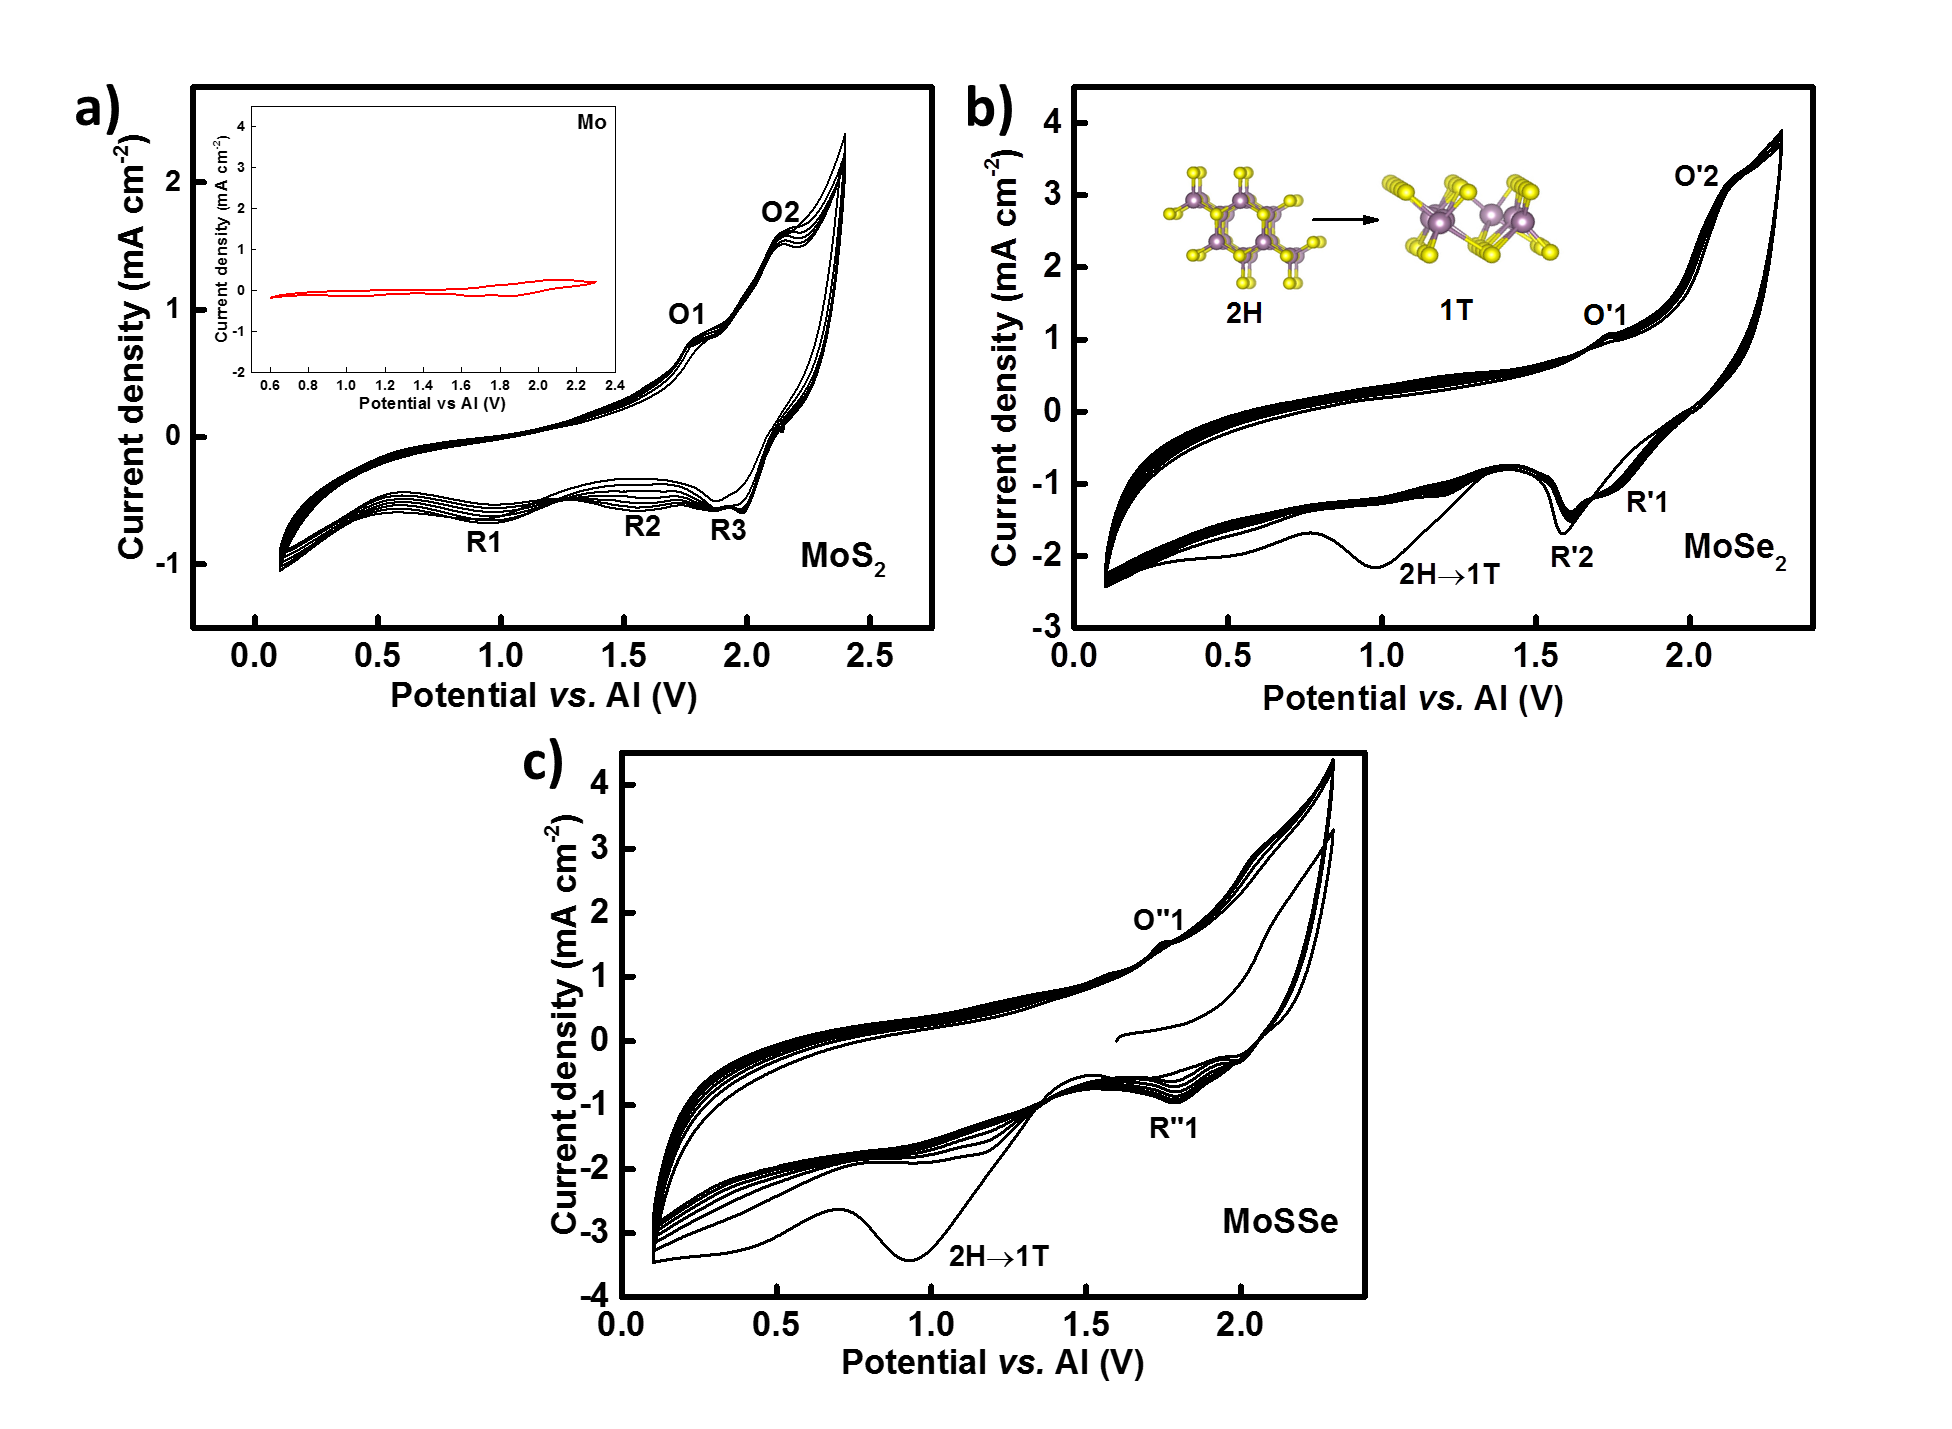
\includegraphics[width=\textwidth]{Figures/chap4fig/fig2}
  \caption{Cyclic voltammograms of a) \ce{MoS2}, b) \ce{MoSe2} and c) MoSSe at a scan rate of 10 mV s$^{-1}$ in a two-electrode aluminium-ion cell against an Al/\ce{Al^{3+}} reference electrode.}
  \label{Figures/chap4fig:fig2}
\end{figure} 

\begin{figure}
  \centering
  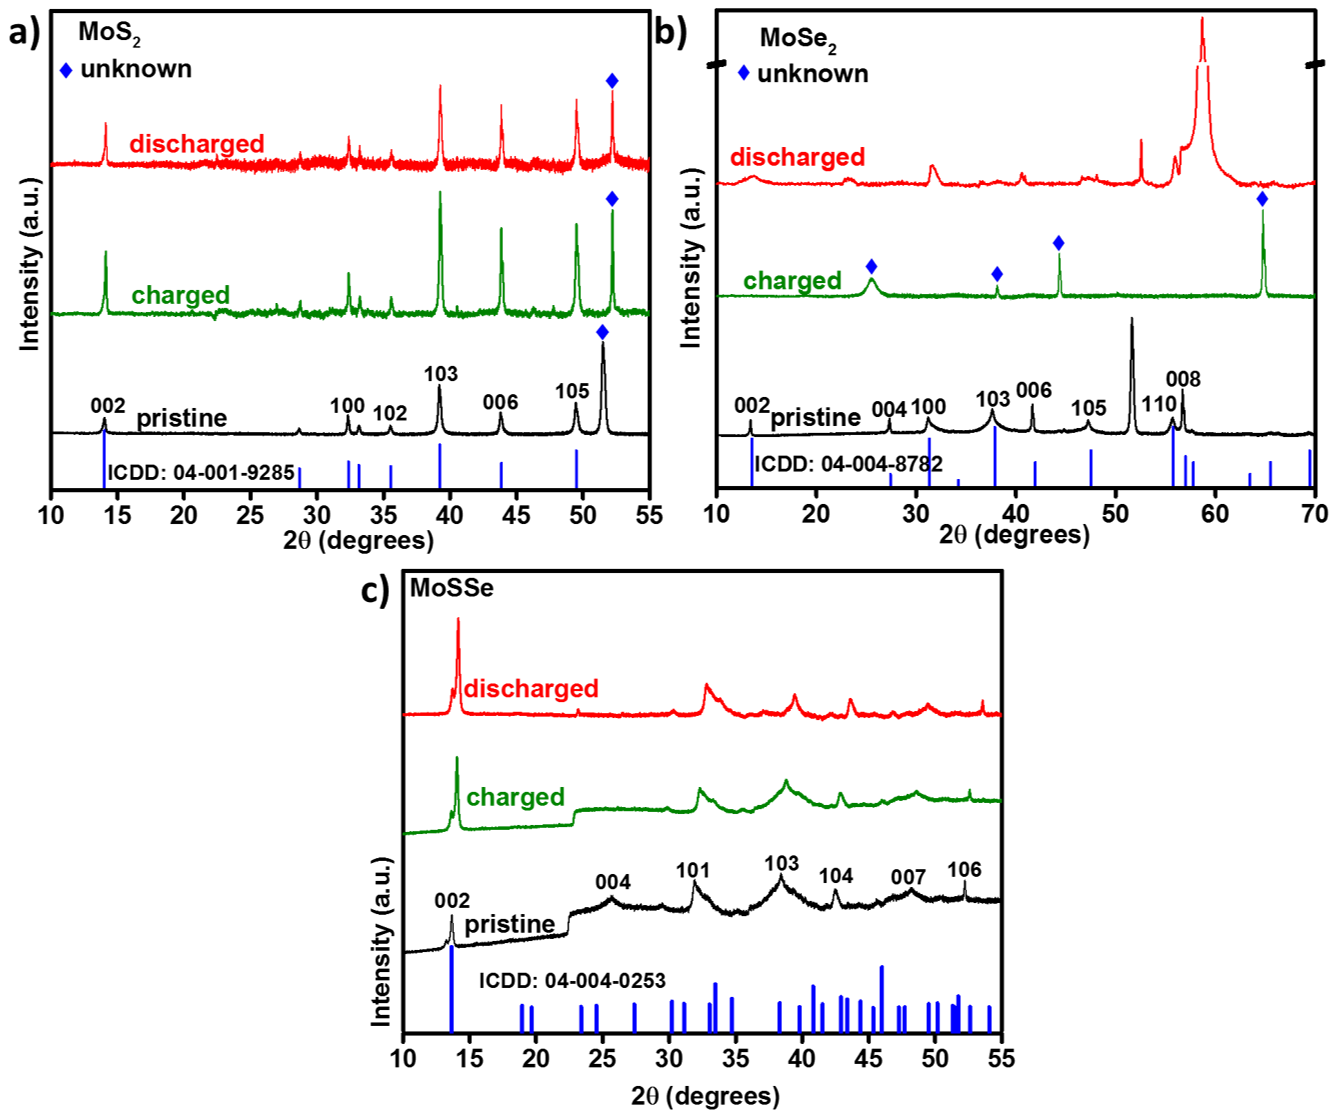
\includegraphics[width=\textwidth]{Figures/chap4fig/fig3}
  \caption{X-ray diffraction patterns of pristine (black), charged (green) and discharged (red) a) \ce{MoS2}, b) \ce{MoSe2} and c) MoSSe electrodes charged to 2.35 V and discharged to 0.2 V vs. Al/\ce{Al^{3+}}, with International Centre for Diffraction Data (ICDD) references.}
  \label{Figures/chap4fig:fig3}
\end{figure}

Figure \ref{Figures/chap4fig:fig3} shows the XRD patterns of \ce{MoS2}, \ce{MoSe2} and MoSSe electrodes. Pristine (in black), charged (in green) and discharged (in red) cathodes were compared after 30 cycles. \ce{MoS2} cells displayed a very small shift in their d-spacings. The peak at 14.2$^{\circ}$ (6.22 \AA) shifted to 14.02$^{\circ}$ (6.32 \AA), as shown in Figure \ref{Figures/chap4fig:fig3} a). Most of the peaks retained their positions after charge and discharge showing no significant change in the lattice dimensions. A completely different XRD pattern appeared after charging for Al/\ce{MoSe2} cells, as new peaks appeared at 2$\theta$ values, displayed in Figure \ref{Figures/chap4fig:fig3} b). After discharge, the diffraction patterns of the discharged cathodes resembled the pristine cathode patterns. Every time the cells were charged, \ce{MoSe2} seemed to adopt this new crystal lattice. However, the characteristic peaks of \ce{MoSe2} reappeared after discharge. This follows closely the observations made by Rani \textit{et al.} \cite{rani_fluorinated_2013}, where they proved intercalation of ions into the layers of fluorinated natural graphite during charging. This strongly confirms our hypothesis of a reversible intercalation taking place in \ce{MoSe2}. It was interesting to note that MoSSe did not have a well-defined crystal structure to begin with, Figure \ref{Figures/chap4fig:fig3} c). The patterns after charge and discharge did not look any different from the untested cathode. This confirmed MoSSe layers did not undergo any expansion and the initial specific capacities came from non-faradaic reactions where \ce{AlCl4-} might have been electrostatically absorbed and desorbed onto the surface of the electrode.  

To further understand the interactions between \ce{AlCl4-} and \ce{MoSe2} we used XPS, which is a useful method for distinguishing various oxidation states and helps in identifying different polymorphs (2H and 1T) \cite{fan_hybrid_2017}. The detailed narrow spectrum scans in Figure \ref{Figures/chap4fig:MoAlOverallMoSeMoSSe} show the binding energies of Mo (3d$_{5/2}$ and 3d$_{3/2}$, Figure \ref{Figures/chap4fig:MoAlOverallMoSeMoSSe} a) and b)) and Al 2p peaks for charged \ce{MoSe2} (Figure \ref{Figures/chap4fig:MoAlOverallMoSeMoSSe} c)) and MoSSe electrodes (Figure \ref{Figures/chap4fig:MoAlOverallMoSeMoSSe} d)). In pristine \ce{MoSe2}, two peaks appeared at 229.1 eV and 232.2 eV corresponding to 3d$_{5/2}$ and 3d$_{3/2}$ (Figure\ \ref{Figures/chap4fig:MoSeSeAlClPrtChg} a)). Selenium displayed a doublet at 55.4 eV and 54.6 eV corresponding to Se 3d$_{3/2}$ and 3d$_{5/2}$ respectively (Figure \ref{Figures/chap4fig:MoSeSeAlClPrtChg} c)). Peak splitting in an XPS spectrum can indicate a phase change or a change in oxidation state. After charge, the peak for Mo 3d split into three doublets indicating the presence of multiple oxidation states or phases of Mo (Figure \ref{Figures/chap4fig:MoAlOverallMoSeMoSSe} a)). Se 3d deconvoluted into four peaks after charge, Figure \ref{Figures/chap4fig:MoSeSeAlClPrtChg} e), confirming presence of more than one phase after charge. This was similar to observations made by Fan \textit{et al.} Pristine electrodes of MoSSe contained Mo in more than one oxidation state, and provided evidence for the presence of both 2H and 1T polymorphs, Figure\ \ref{Figures/chap4fig:MoSeSeAlClPrtChg} b). After charging, the width of peaks at 231.7 eV (Mo 3d$_{5/2}$) and 228.6 eV (Mo 3d$_{3/2}$) increased as displayed in Figure\ \ref{Figures/chap4fig:MoAlOverallMoSeMoSSe} b). After comparing Figure\ \ref{Figures/chap4fig:MoSeSeAlClPrtChg} d) and f), we noticed that the Se 3d spectrum deconvoluted into four peaks after charging in MoSSe cells. An increase in the peak width was observed for both Mo and Se binding energies. A new peak at $\sim$236 eV in Mo 3d spectra for \ce{MoS2}, \ce{MoSe2} and MoSSe electrodes generally indicates a Mo$^{6+}$ species present in molybdenum oxide, \ce{MoO3}. 

\begin{figure}
  \centering
  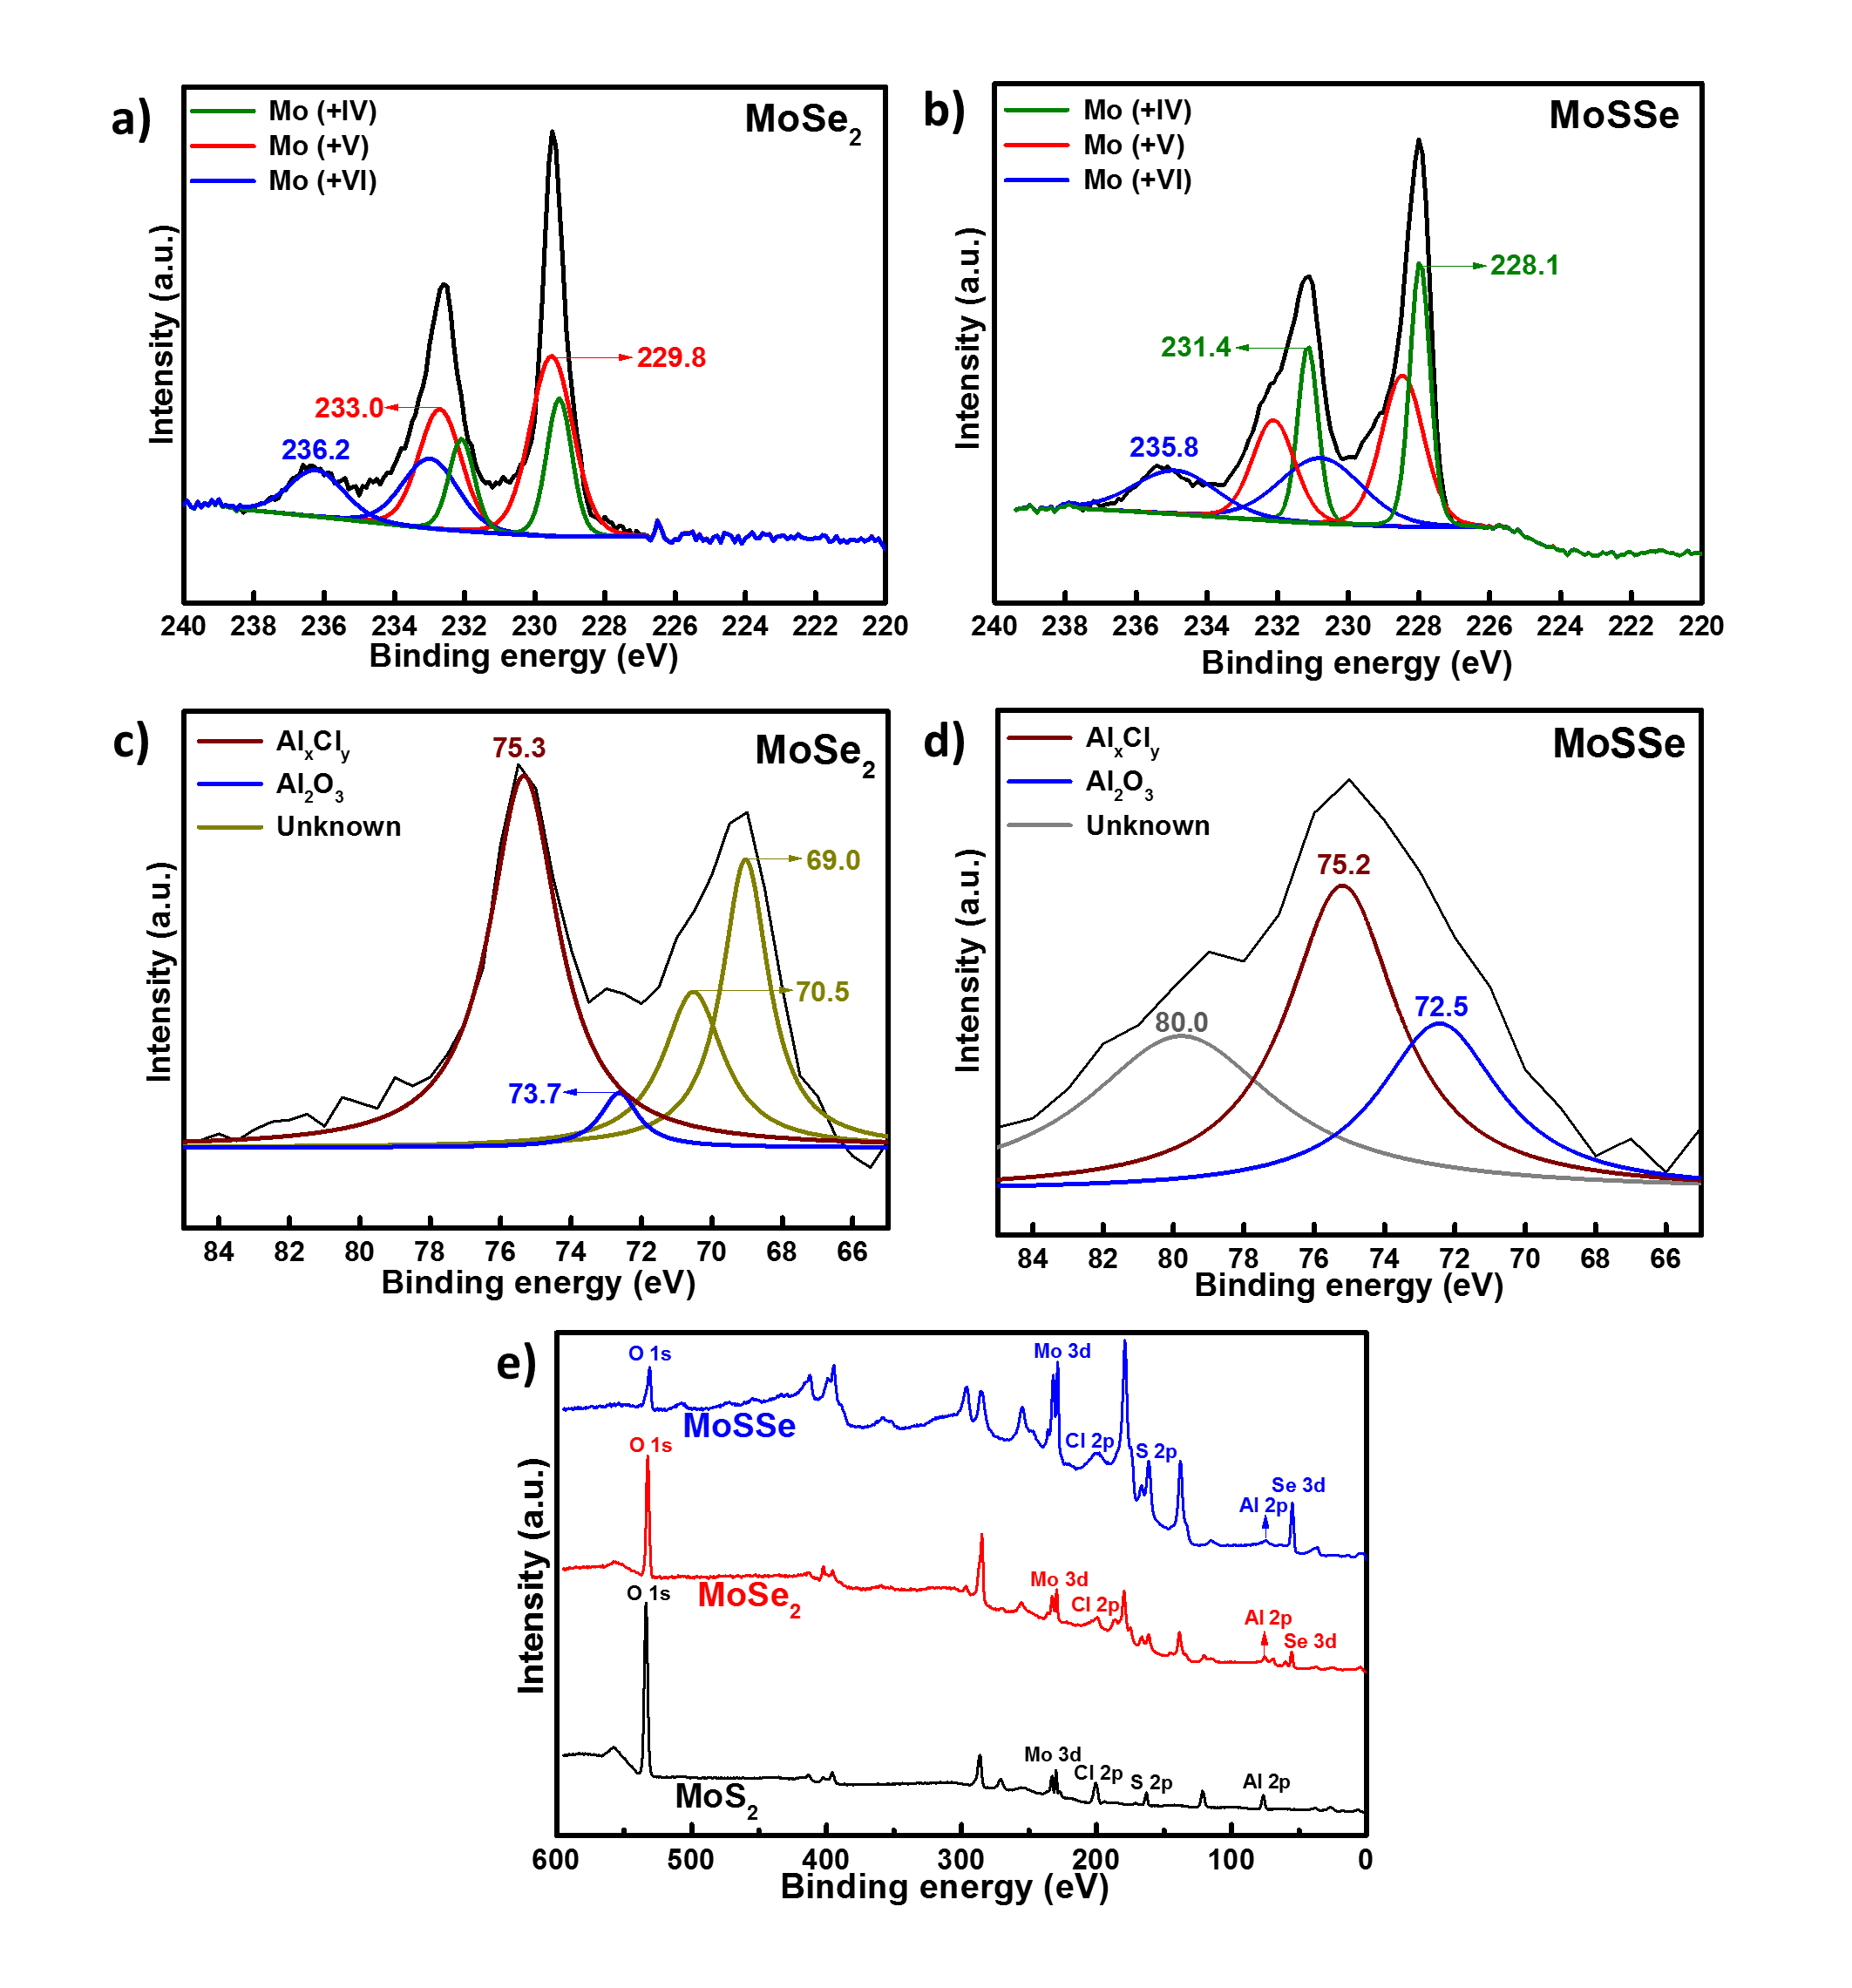
\includegraphics[width=\textwidth]{Figures/chap4fig/MoAlOverallMoSeMoSSe}
  \caption{XPS spectra of Mo 3d orbitals in a charged a) \ce{MoSe2} and b) MoSSe cathode and Al 2p orbitals in a charged c) \ce{MoSe2} and d) MoSSe cathode. e) An overview spectrum of all three tested and charged cathodes.}
  \label{Figures/chap4fig:MoAlOverallMoSeMoSSe}
\end{figure}

The peak shifts detected in Mo 3d spectra for charged \ce{MoS2} and \ce{MoSe2} cathodes were insignificant in MoSSe (cf.\ Figures \ref{Figures/chap4fig:MoS2XPS} a), b), \ref{Figures/chap4fig:MoAlOverallMoSeMoSSe} a), and \ref{Figures/chap4fig:MoSeSeAlClPrtChg} a)). This further confirms the absence of redox reactions and that the capacity was mainly derived from a surface-based charge storage. As expected, charged electrodes showed higher concentration of aluminium and chlorine than discharged electrodes as seen in Figure \ref{Figures/chap4fig:MoSeSeAlClPrtChg} g) and h). The XPS spectra support the observation that \ce{MoSe2} underwent a phase transformation that made it a better performing cathode than \ce{MoS2}. Further analysis is needed to fully understand the mechanism of MoSSe.

\begin{figure}
  \centering
  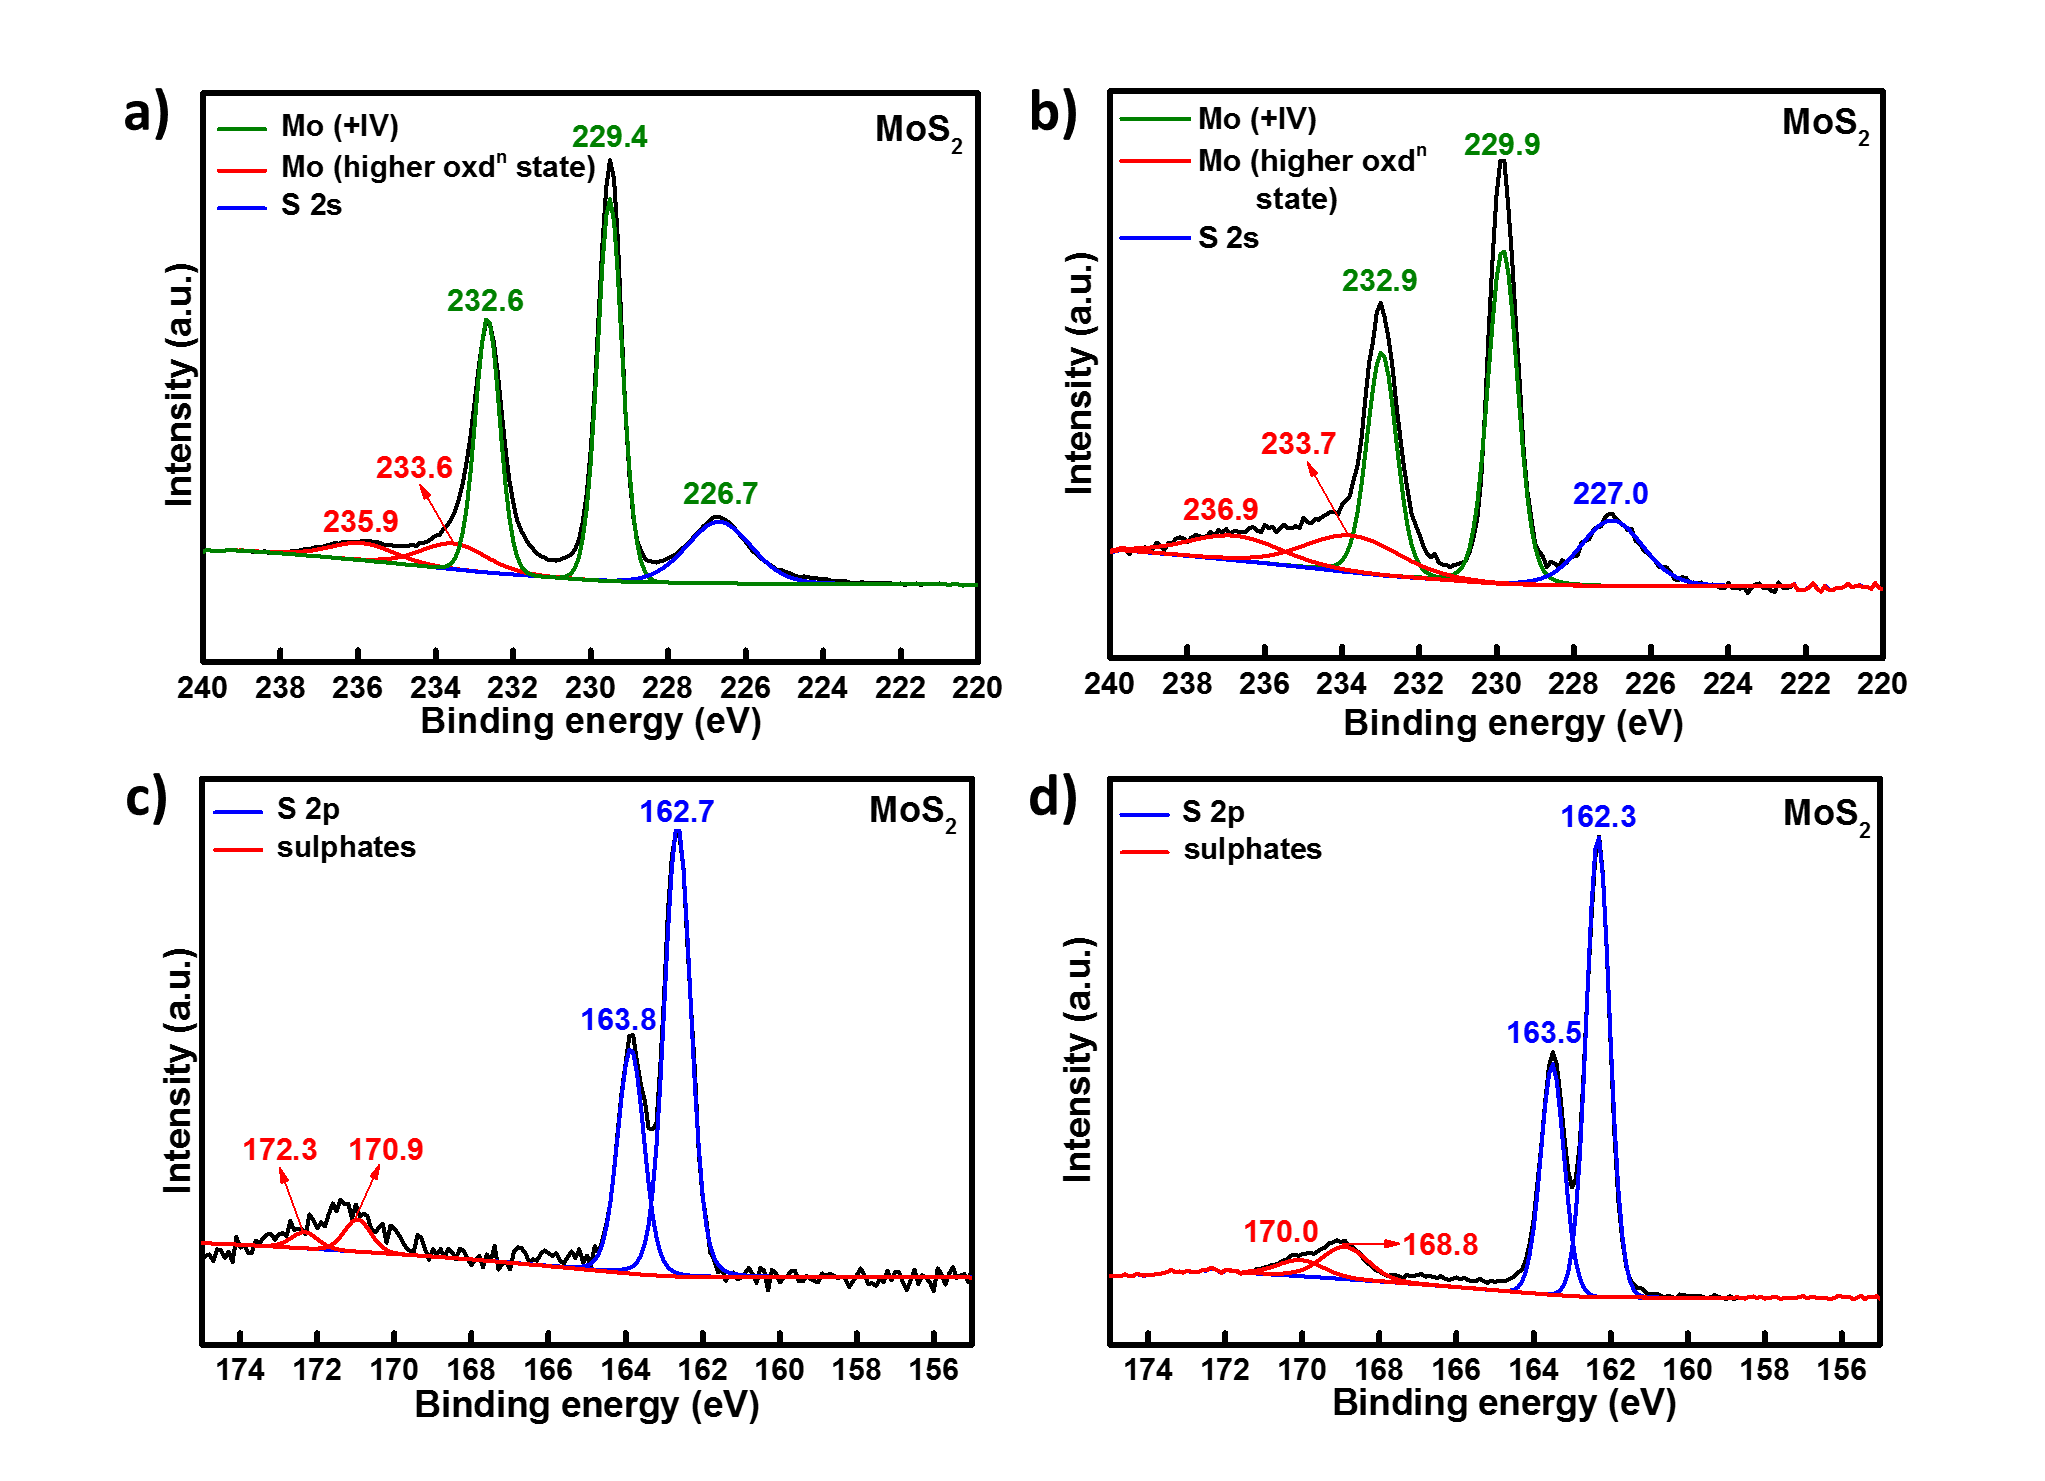
\includegraphics[width=\textwidth]{Figures/chap4fig/MoS2XPS}
  \caption{XPS spectra of Mo 3d orbitals in a charged and b) discharged \ce{MoS2} cathode and binding energies of S 2p orbital in a charged and b) discharged \ce{MoS2} cathode.}
  \label{Figures/chap4fig:MoS2XPS}
\end{figure}

\begin{figure}
  \centering
  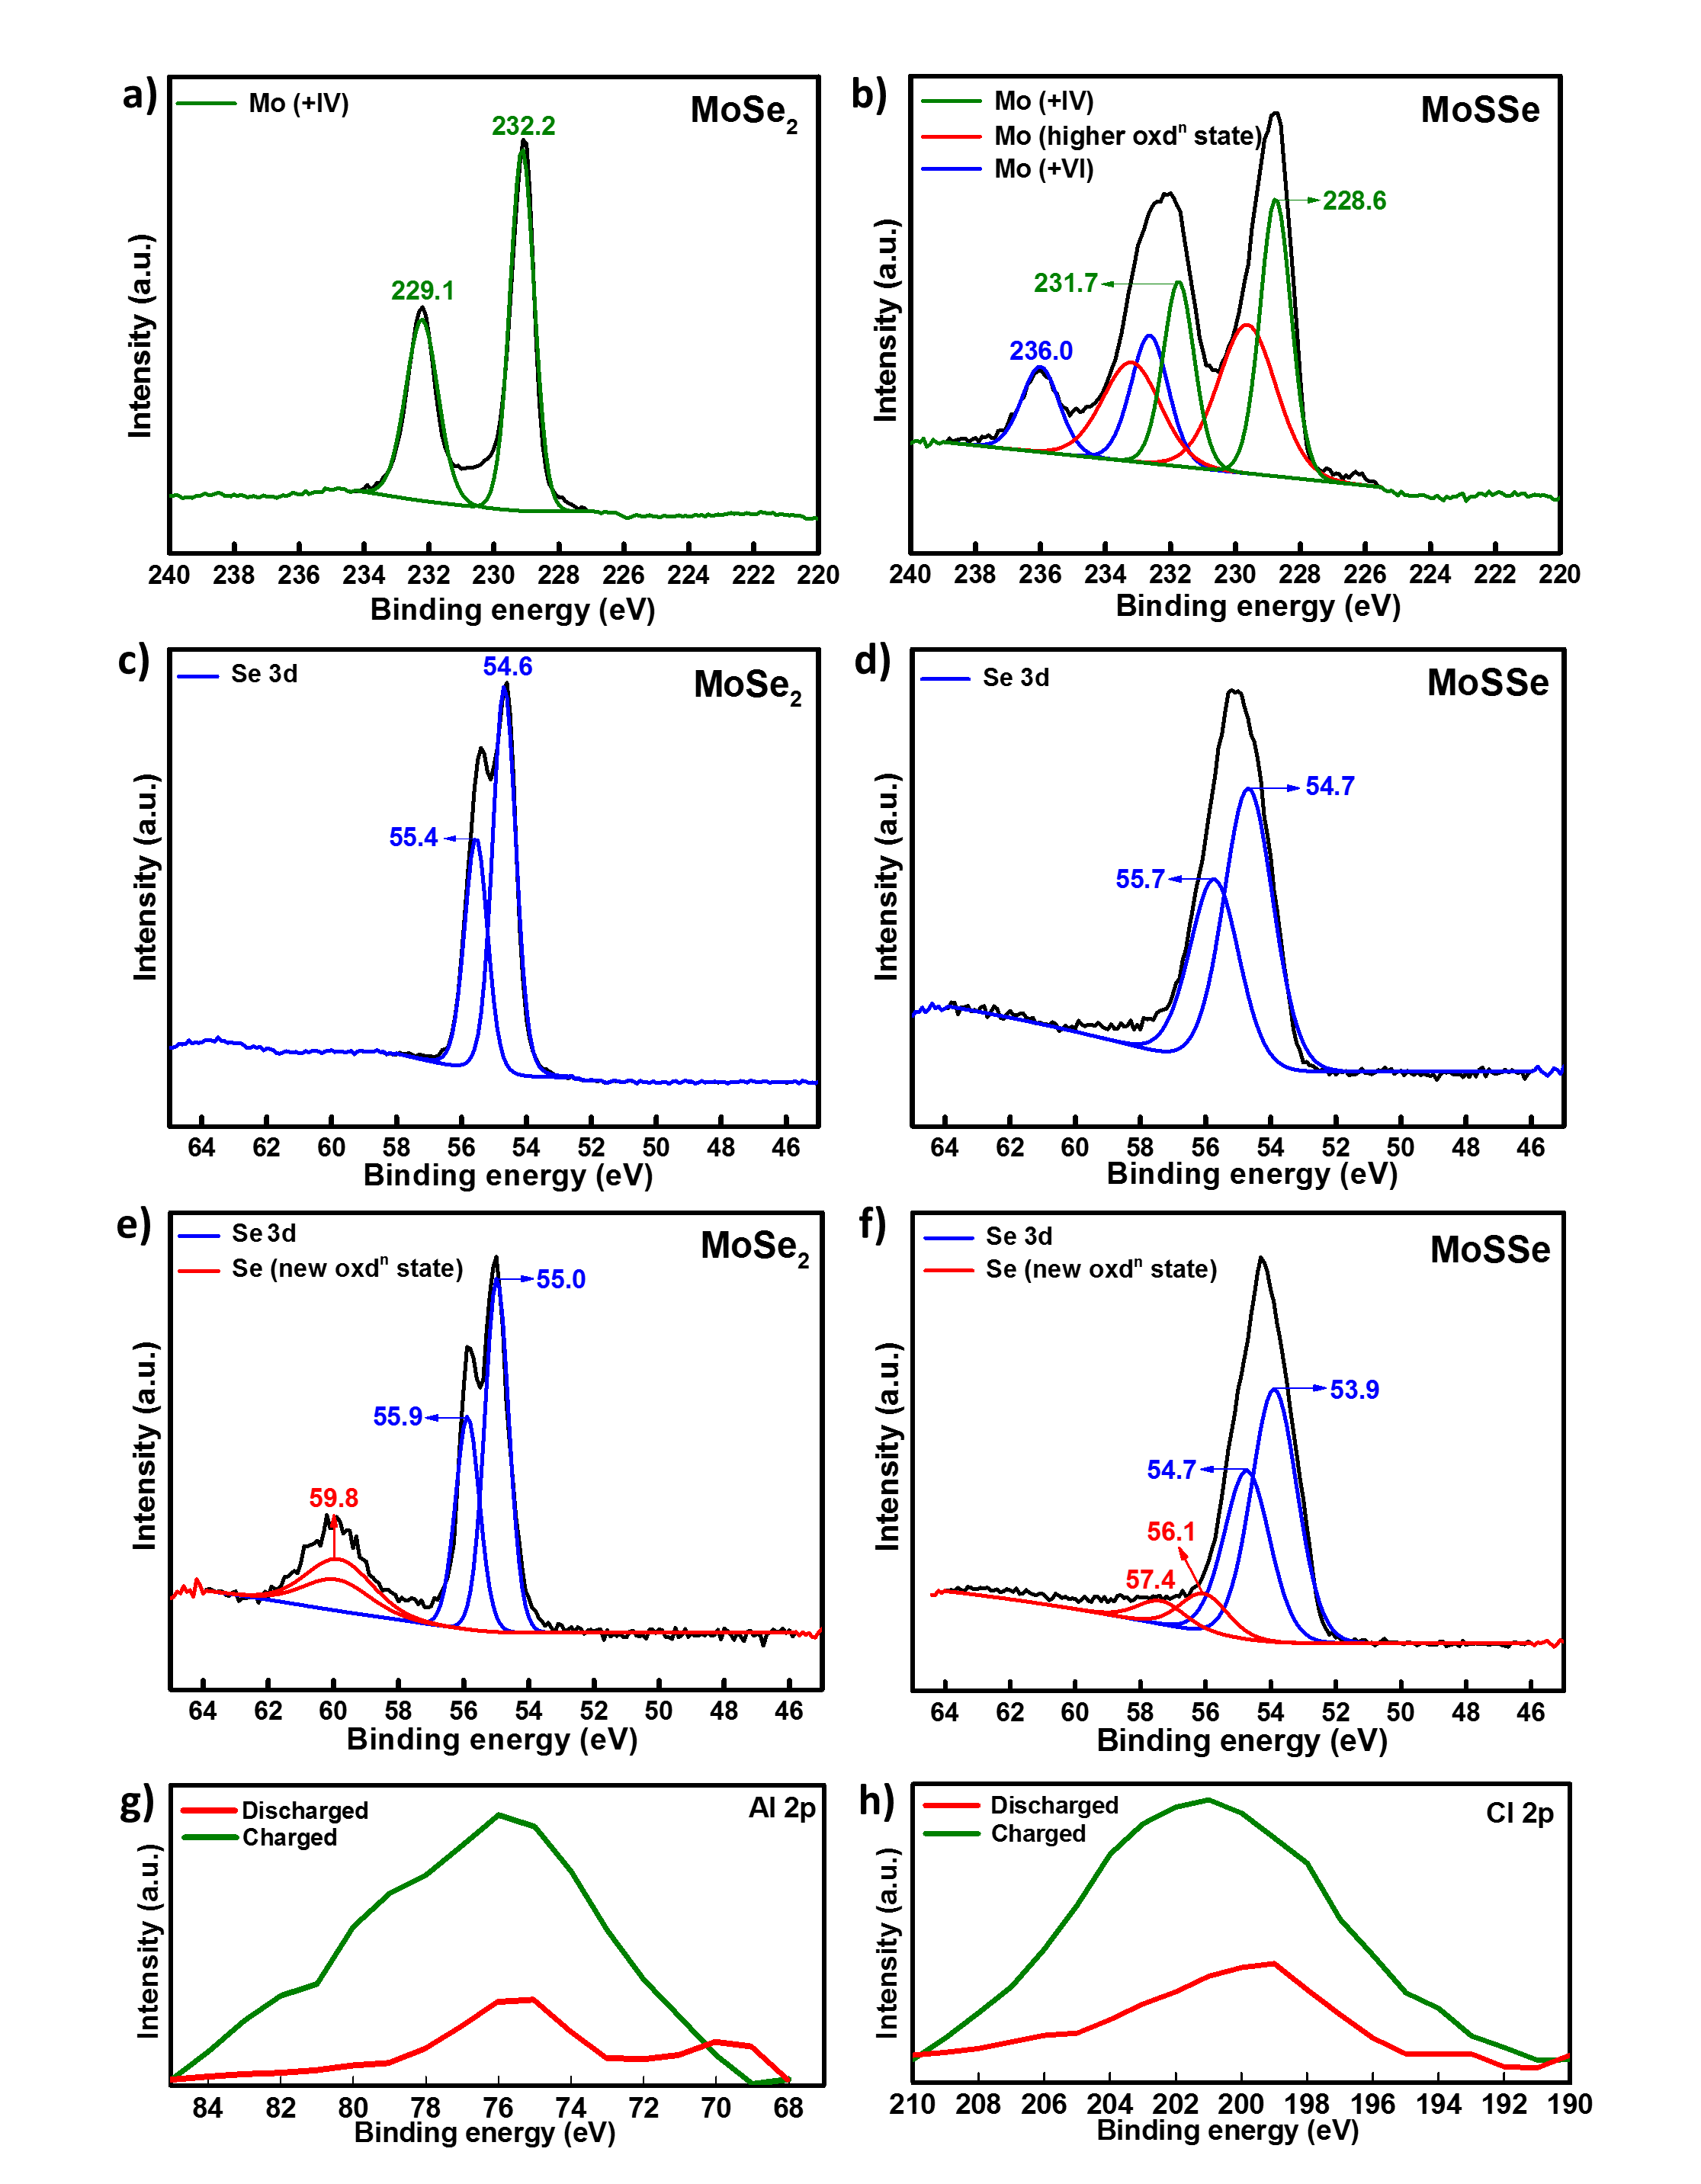
\includegraphics[width=\textwidth]{Figures/chap4fig/MoSeSeAlClPrtChg}
  \caption{XPS spectra of Mo 3d for pristine a) \ce{MoSe2} and b) MoSSe electrodes. The spectra of \ce{MoSe2} are composed of two peaks at 232.2 eV and 229.1 eV corresponding to \ce{Mo^{4+}}. MoSSe spectra consist of three doublet bands, which were assigned to \ce{Mo^{4+}}, one with higher oxidation state and another band corresponding to \ce{Mo^{6+}} at 236 eV. c) Pristine and e) charged Se 3d from \ce{MoSe2}. \ce{MoSe2} observed peaks corresponding to 3d$_{3/2}$ and 3d$_{5/2}$ at 55.6 eV and 54.6 eV respectively. Binding energies of Se 3d from d) pristine and f) charged MoSSe cathodes.}
  \label{Figures/chap4fig:MoSeSeAlClPrtChg}
\end{figure}

Charged \ce{MoSe2} electrodes displayed binding energies of Al 2p at 77 eV (red) and 76 eV (in blue) corresponding to chlorides (\ce{AlxCly}) and \ce{Al2O3} respectively in Figure \ref{Figures/chap4fig:MoAlOverallMoSeMoSSe} c). New peaks were observed at much lower binding energies --- 69 and 70 eV (green) suggesting the presence of a new complex with an increased electron density around aluminium. An overall spectra of charged \ce{MoS2}, \ce{MoSe2} and MoSSe cathodes is shown in Figure \ref{Figures/chap4fig:MoAlOverallMoSeMoSSe} e) indicating the presence of Al and Cl (from chloroaluminates) and oxygen (from \ce{MoO3}).

In addition, we compared the Raman spectra of pristine and charged cathodes to detect shifts in vibrational modes, Figure \ref{Figures/chap4fig:fig5}. E$^1_{2g}$ and A$^1_g$ are the most intense vibrational modes for molybdenum dichalcogenides \cite{yang_pressure-induced_2019,sharma_stable_2018}. Peaks corresponding to E$^1_{2g}$ and A$^1_g$ modes for \ce{MoS2} (Figure \ref{Figures/chap4fig:fig5} a)) are prominent at 384.6 cm$^{-1}$ and 410.2 cm$^{-1}$ respectively. A$^1_g$ indicates an out-of-plane symmetric displacement of S atoms, whereas E$^1_{2g}$ suggests an in-layer displacement. Also, separation between the two peaks indicates a multi-layer structure, which was observed for all three materials. No significant peak shift or peak broadening was observed for the charged \ce{MoS2} electrode. For 2H \ce{MoSe2} (Figure \ref{Figures/chap4fig:fig5} b)), A$^1_g$ is the most intense vibration occurring at a frequency lower than that of E$^1_{2g}$. When the number of layers decreases, the A$^1_g$ mode softens (increase in full-width-at-half-maximum (FWHM)). Spectra generated after intercalation were different from the pristine cathodes because phase conversion from 2H to 1T decreases the molecule's symmetry and more Raman bands get active. The presence of J1 and J2 peaks in addition to E$^1_{2g}$ and A$^1_g$ at lower wavelengths suggest the existence of 1T phase especially for \ce{MoSe2} and MoSSe (inset, Figure\ \ref{Figures/chap4fig:fig5} b) and c)). This agrees with our CV scans where a phase transition was observed for \ce{MoSe2} and MoSSe. Raman results suggest that 'chloroalumination' or insertion of chloroaluminates changed the symmetry and vibrational modes of \ce{MoSe2}'s crystal lattice. 

\begin{figure}
  \centering
  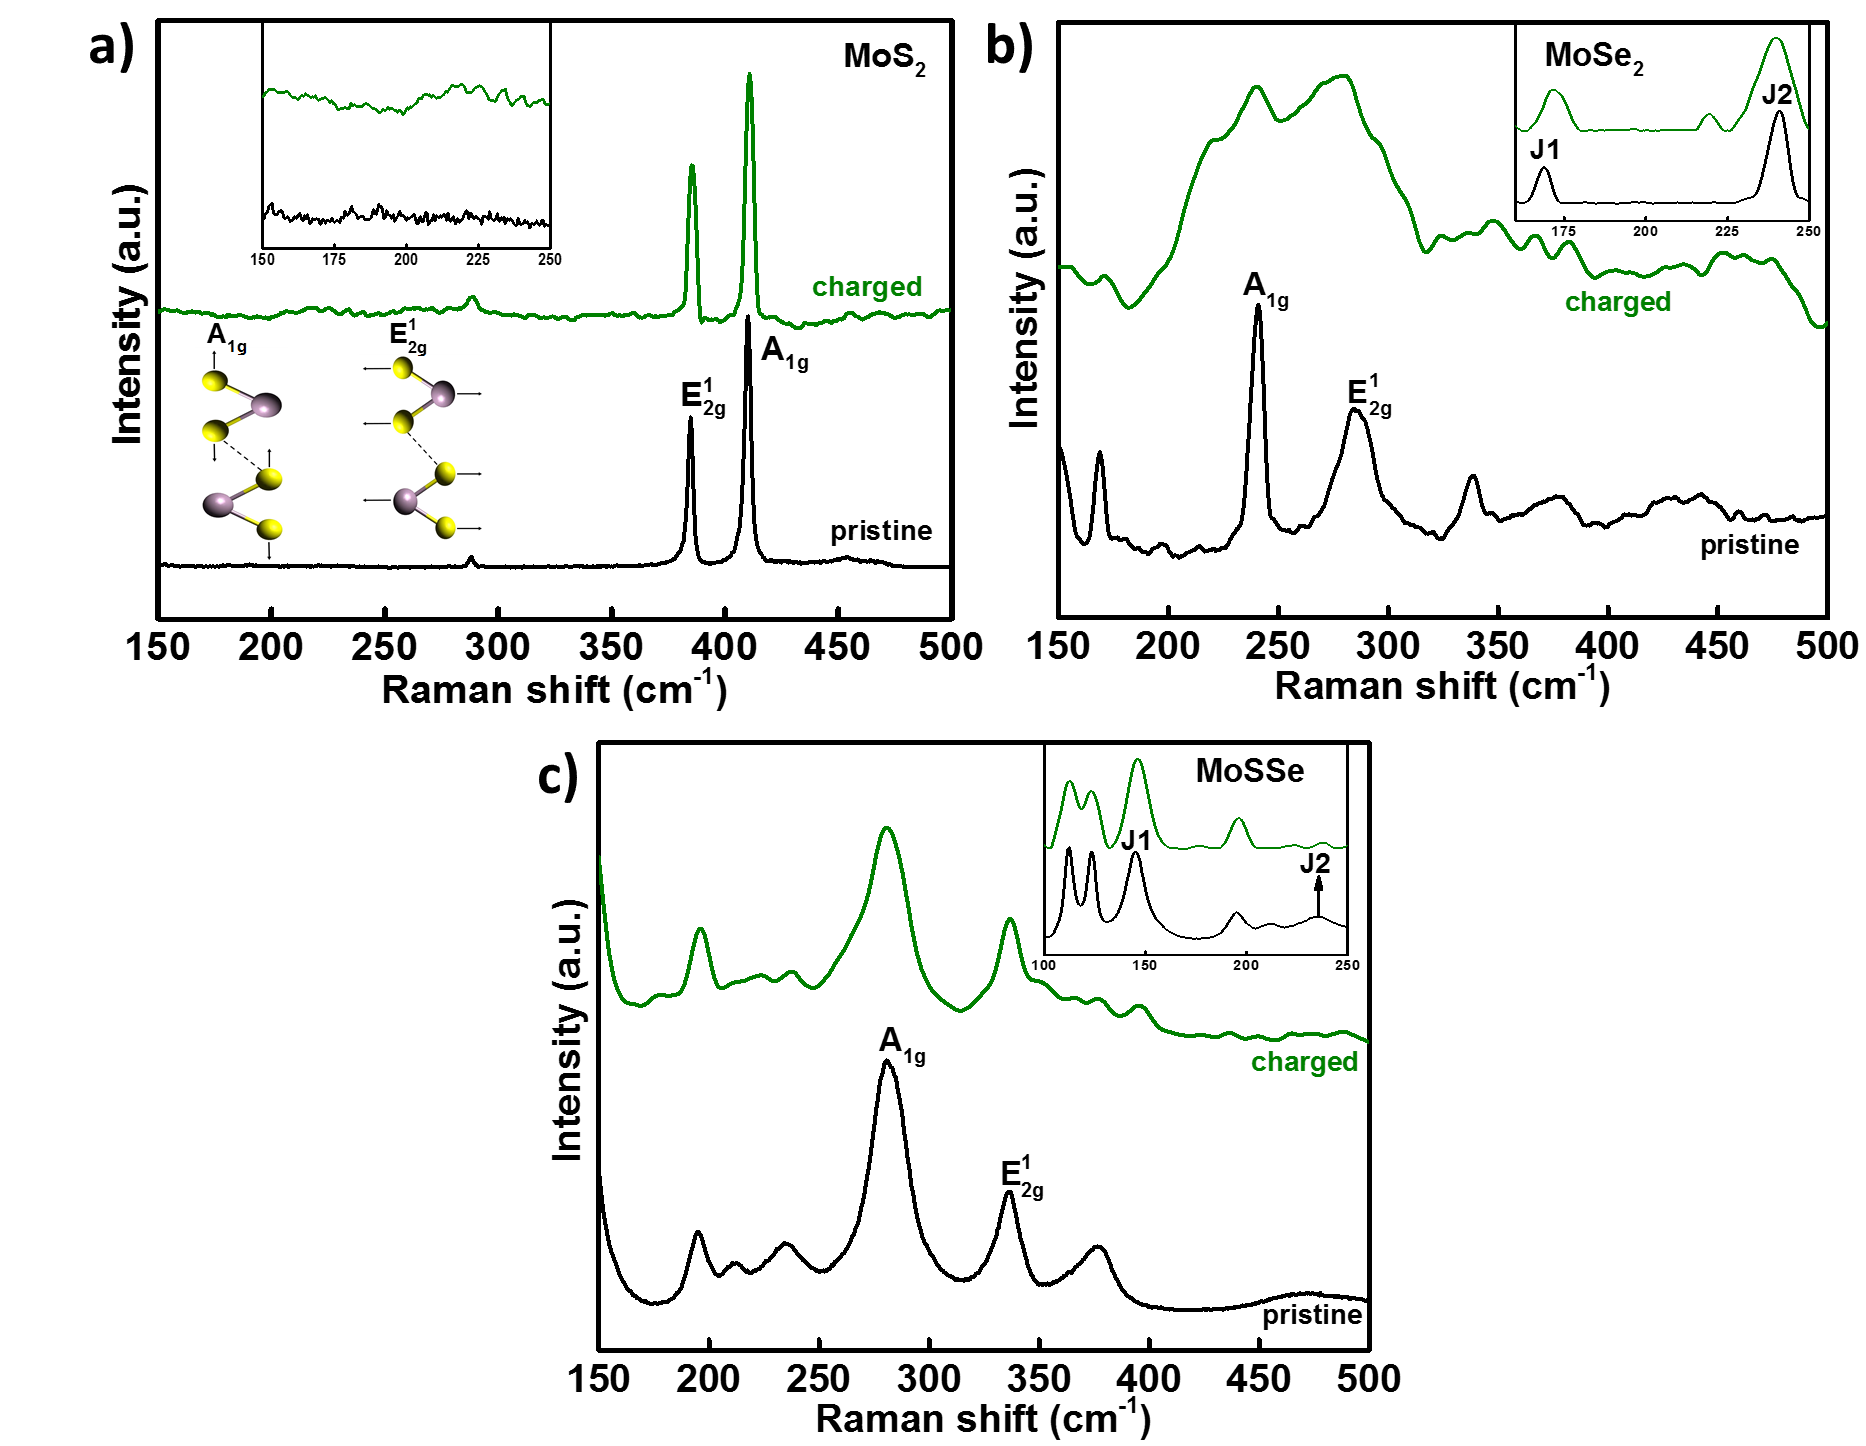
\includegraphics[width=\textwidth]{Figures/chap4fig/fig5}
  \caption{Raman spectra of pristine (black) and charged (green) a)\ce{MoS2}, b) \ce{MoSe2} and c) MoSSe electrodes with position of new Raman active J1 and J2 bands marked along with E$^1_{2g}$ and A$^1_g$ bands.}
  \label{Figures/chap4fig:fig5}
\end{figure}

\begin{figure}
  \centering
  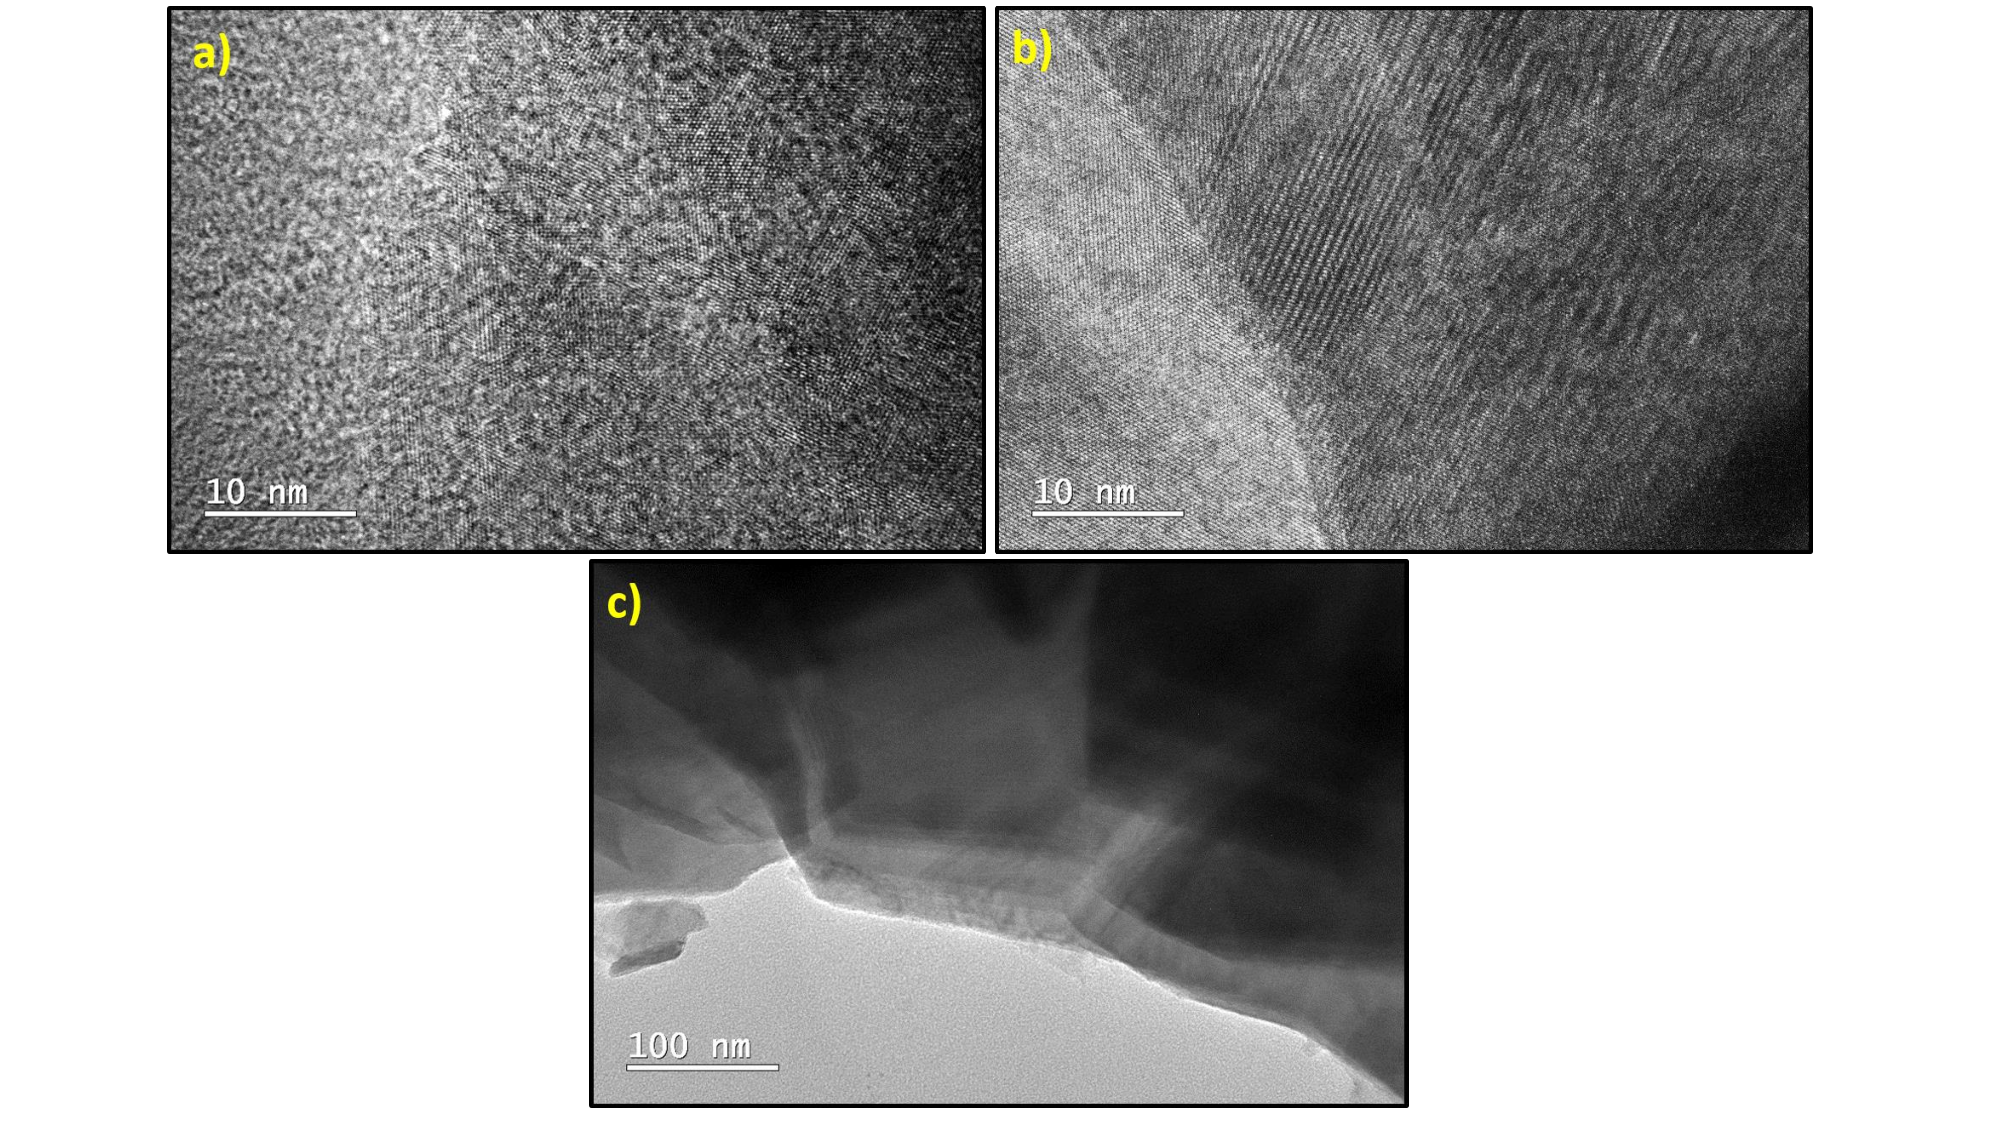
\includegraphics[width=\textwidth]{Figures/chap4fig/mose2tem}
  \caption{Raman spectra of pristine (black) and charged (green) a)\ce{MoS2}, b) \ce{MoSe2} and c) MoSSe electrodes with position of new Raman active J1 and J2 bands marked along with E$^1_{2g}$ and A$^1_g$ bands.}
  \label{Figures/chap4fig:mose2tem}
\end{figure}
